\documentclass{article}

\usepackage{enumerate}
\usepackage{amssymb}
\usepackage{amsmath}
\usepackage{algorithm}
\usepackage{listings}
\usepackage[noend]{algpseudocode}
\usepackage{graphicx}

\graphicspath{ {./} }

\topmargin=-0.45in
\evensidemargin=0in
\oddsidemargin=0in
\textwidth=6.5in
\textheight=9.0in
\headsep=0.25in

\title{Chem 195: Problem Set 3}
\author{Michael Stephen Chen}


\begin{document}
\maketitle
\pagebreak

\section*{Problem 1}
\begin{enumerate}[i.]
  \item See \textit{ho.m} for all my added comments
  \item The following are the calculatedenergies for the 9 lowest energy levels. To reprodue these results, run the first section of \textit{HOConverge1D.m}\\
    \begin{center}
    $\begin{array}{c|c}
      Level & Energy (\epsilon)  \\ \hline
      0 & 0.5001 \\
      1 & 1.5021 \\
      2 & 2.5176 \\
      3 & 3.5944 \\
      4 & 4.8016 \\
      5 & 6.2846 \\
      6 & 8.0551 \\
      7 & 10.4124\\
      8 & 13.4974
    \end{array}$\\
    \end{center}

  \item Below is a plot showing the convergence of energy levels with increasing number of basis functions $K$. Qualitatively, it appears that convergence is achieved for the lowest nine levels around $K=15$

    \begin{center}
      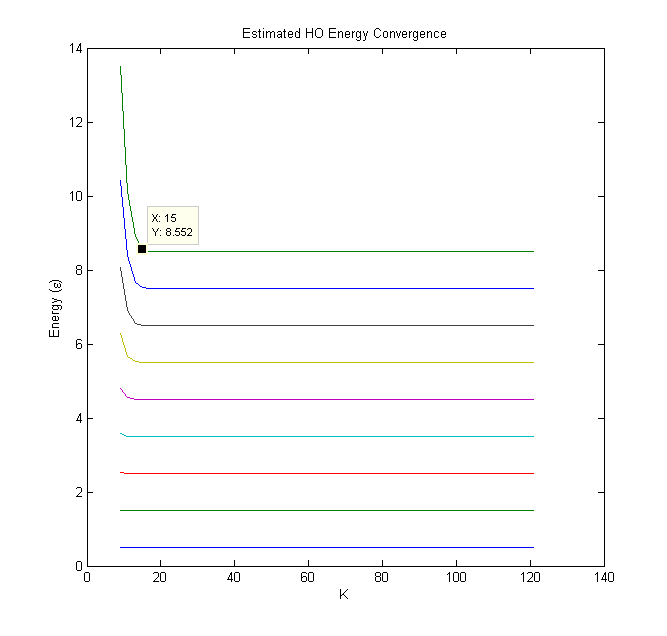
\includegraphics[scale=0.5]{prob1part3}
    \end{center}

\end{enumerate}


\section*{Problem 2}
\begin{enumerate}[i.]
  \item 
    \begin{align*}
      H\psi &= \left[ -\frac{1}{2} \left(  \frac{d^2}{dx^2} + \frac{d^2}{dy^2} \right) + \frac{1}{2} (x^2 + y^2) \right] \left( \psi_x \psi_y \right) \\
      &= \frac{1}{2} \left(  -\frac{d^2}{dx^2} + x^2 \right) \left( \psi_x \psi_y \right) + \frac{1}{2} \left(  -\frac{d^2}{dy^2} + y^2 \right) \left( \psi_x \psi_y \right) \\
      &= \psi_y \left[  \frac{1}{2} \left(  -\frac{d^2}{dx^2} + x^2\right) \psi_x \right] + \psi_x \left[  \frac{1}{2} \left(  -\frac{d^2}{dy^2} + y^2\right) \psi_y \right] \\
      &= \psi_y E_x \psi_x + \psi_x E_y \psi_y \\
      &= \left( E_x + E_y \right) \psi_x \psi_y
    \end{align*}

  \item The following is the equation for the energy of the 2D-HO given $n_x$ and $n_y$ where $n_x , n_y \in \mathbb{N}$
    \begin{align*}
      E &= E_x + E_y \\
      &= (n_x + 1/2) + (n_y + 1/2) \\
      &= n_x + n_y + 1
    \end{align*}
    An enumeration of the first couple energy states $n=n_x + n_y$ is presented below. In general the number of degeneracies is equivalent to $n+1$

    \begin{center}
    $\begin{array}{ccc|c}
      n & n_x & n_y & Energy (\epsilon)  \\ \hline
      0 & 0 & 0 & 1 \\ \hline
      1 & 1 & 0 & 2 \\
        & 0 & 1 &   \\ \hline
      2 & 1 & 1 & 3 \\
        & 2 & 0 &   \\
        & 0 & 2 &   \\ \hline
    \end{array}$\\
    \end{center}    
\end{enumerate}

\pagebreak

\section*{Problem 3}
Below is the code from \textit{harmOsc2DEnergies.m}\\
\lstinputlisting[frame=single]{harmOsc2DEnergies.m}

\pagebreak

\section*{Problem 4}
\begin{enumerate}[i.]
  \item Below are the calculated energies for the 45 lowest energy eigenstatess for $K=49$ basis fns. The results can be reproduced by running the first section of \textit{HOConverge2D.m}. The result for the ground state and the first excited statess are fairly close to the theoretical values of 1 and 2, respectively. Also we can see the degeneracy of the first excited state. However with increassing energy levels the calculated value deviate more and more.
    \begin{center}
    $\begin{array}{c|c}
      index & Energy (\epsilon) \\ \hline
      1 & 1.0036 \\ 
      2 & 2.0291 \\ 
      3 & 2.0291 \\ 
      4 & 3.0545 \\ 
      5 & 3.1434 \\ 
      6 & 3.1434 \\ 
      7 & 4.1688 \\ 
      8 & 4.1688 \\ 
      9 & 4.5276 \\ 
      10 & 4.5276 \\ 
      11 & 5.2831 \\ 
      12 & 5.5531 \\ 
      13 & 5.5531 \\ 
      14 & 6.2278 \\ 
      15 & 6.2278 \\ 
      16 & 6.6674 \\ 
      17 & 6.6674 \\ 
      18 & 7.2532 \\ 
      19 & 7.2532 \\ 
      20 & 8.0516 \\ 
      21 & 8.3675 \\ 
      22 & 8.3675 \\ 
      23 & 8.6903 \\ 
      24 & 8.6903 \\ 
      25 & 9.7158 \\ 
      26 & 9.7158 \\ 
      27 & 9.7518 \\ 
      28 & 9.7518 \\ 
      29 & 10.8301 \\ 
      30 & 10.8301 \\ 
      31 & 11.4519 \\ 
      32 & 11.7807 \\ 
      33 & 11.7807 \\ 
      34 & 12.2143 \\ 
      35 & 12.2143 \\ 
      36 & 12.8061 \\ 
      37 & 12.8061 \\ 
      38 & 13.9145 \\ 
      39 & 13.9145 \\ 
      40 & 13.9205 \\ 
      41 & 13.9205 \\ 
      42 & 15.3047 \\ 
      43 & 15.3047 \\ 
      44 & 16.3770 \\ 
      45 & 17.0049 \\
    \end{array}$
    \end{center}
    \pagebreak

  \item To reproduce the figure below, please run the second section of \textit{HOConverge2D.m}. It appears as though $K=225$ basis are necessary for convergence of the first 9 energy levels for the 2D HO.
    \begin{center}
      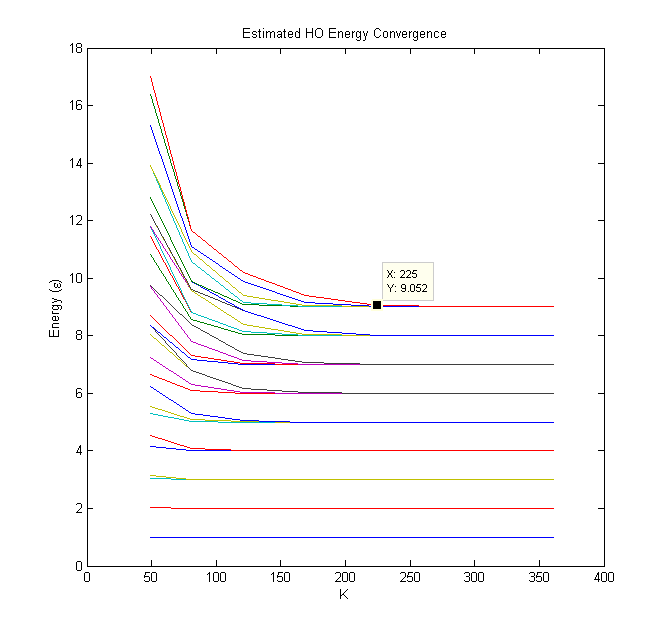
\includegraphics[scale=0.6]{prob4part2.png}
    \end{center}

  \item Given that for the 1D HO we needed around 15 basis fns and we needed apprximately $15^2 = 225$ basis fns for a 2D HO, we would probably need $15^3 = 3375$ basis fns for the first 9 energy levels to converge for a 3D HO. So in general the dimensionality of the wavefn $\psi (x_1, x_2,...,x_N)$ will require roughly $c^N$ basis functions, where $c$ is some constant intrinsic to the problem at hand, or in another words the number of basis functions scale exponentially with the dimensionality of the wavefn/equation we are solving for.

  \item Therefore with N-electron problems in 3D where we have 3N coordinates, the computational expense should be $O(c^{3N})$. So the computational expense grows very quickly with increasing number of electrons, making such calculationss slow/infeasible for large $N$.

\end{enumerate}

\section*{Problem 5}
The wavefunctions were calculated using $K=25$ basis sets. To reproduce the following, run the file \textit{HOWavefnPlot.m}

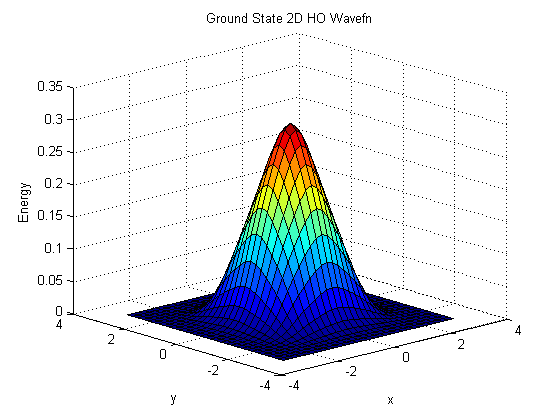
\includegraphics{prob5ground}

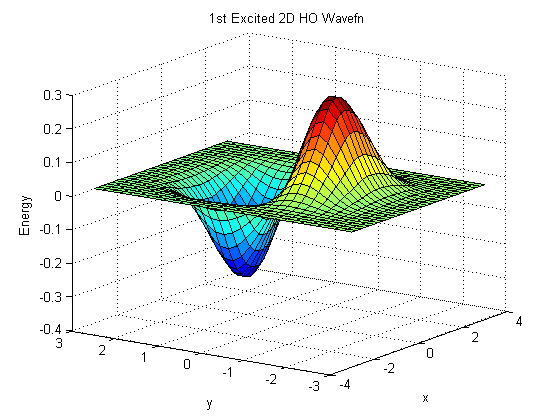
\includegraphics{prob5excited}


\end{document}
